%%%%%%%%%%%%%%%%%%%%%%%%%%%%%%%%%%%%%%%%%
% Beamer Presentation
% LaTeX Template
% Version 2.0 (March 8, 2022)
%
% This template originates from:
% https://www.LaTeXTemplates.com
%
% Author:
% Vel (vel@latextemplates.com)
%
% License:
% CC BY-NC-SA 4.0 (https://creativecommons.org/licenses/by-nc-sa/4.0/)
%
%%%%%%%%%%%%%%%%%%%%%%%%%%%%%%%%%%%%%%%%%

%----------------------------------------------------------------------------------------
%	PACKAGES AND OTHER DOCUMENT CONFIGURATIONS
%----------------------------------------------------------------------------------------

\documentclass[
	11pt, % Set the default font size, options include: 8pt, 9pt, 10pt, 11pt, 12pt, 14pt, 17pt, 20pt
	%t, % Uncomment to vertically align all slide content to the top of the slide, rather than the default centered
	%aspectratio=169, % Uncomment to set the aspect ratio to a 16:9 ratio which matches the aspect ratio of 1080p and 4K screens and projectors
]{beamer}

\graphicspath{{Images/}{./}} % Specifies where to look for included images (trailing slash required)

\usepackage{booktabs} % Allows the use of \toprule, \midrule and \bottomrule for better rules in tables

%----------------------------------------------------------------------------------------
%	SELECT LAYOUT THEME
%----------------------------------------------------------------------------------------

% Beamer comes with a number of default layout themes which change the colors and layouts of slides. Below is a list of all themes available, uncomment each in turn to see what they look like.

% \usetheme{default}
% \usetheme{AnnArbor}
%\usetheme{Antibes}
%\usetheme{Bergen}
%\usetheme{Berkeley}
%\usetheme{Berlin}
%\usetheme{Boadilla}
%\usetheme{CambridgeUS}
%\usetheme{Copenhagen}
%\usetheme{Darmstadt}
% \usetheme{Dresden}
%\usetheme{Frankfurt}
% \usetheme{Goettingen}
%\usetheme{Hannover}
%\usetheme{Ilmenau}
%\usetheme{JuanLesPins}
% \usetheme{Luebeck}
\usetheme{Madrid}
%\usetheme{Malmoe}
% \usetheme{Marburg}
%\usetheme{Montpellier}
%\usetheme{PaloAlto}
%\usetheme{Pittsburgh}
%\usetheme{Rochester}
% \usetheme{Singapore}
%\usetheme{Szeged}
%\usetheme{Warsaw}

%----------------------------------------------------------------------------------------
%	SELECT COLOR THEME
%----------------------------------------------------------------------------------------

% Beamer comes with a number of color themes that can be applied to any layout theme to change its colors. Uncomment each of these in turn to see how they change the colors of your selected layout theme.

% \usecolortheme{albatross}
% \usecolortheme{beaver}
% \usecolortheme{beetle}
% \usecolortheme{crane}
% \usecolortheme{dolphin}
% \usecolortheme{dove}
% \usecolortheme{fly}
% \usecolortheme{lily}
% \usecolortheme{monarca}
% \usecolortheme{seagull}
% \usecolortheme{seahorse}
% \usecolortheme{spruce}
% \usecolortheme{whale}
% \usecolortheme{wolverine}

%----------------------------------------------------------------------------------------
%	SELECT FONT THEME & FONTS
%----------------------------------------------------------------------------------------

% Beamer comes with several font themes to easily change the fonts used in various parts of the presentation. Review the comments beside each one to decide if you would like to use it. Note that additional options can be specified for several of these font themes, consult the beamer documentation for more information.

\usefonttheme{default} % Typeset using the default sans serif font
%\usefonttheme{serif} % Typeset using the default serif font (make sure a sans font isn't being set as the default font if you use this option!)
%\usefonttheme{structurebold} % Typeset important structure text (titles, headlines, footlines, sidebar, etc) in bold
%\usefonttheme{structureitalicserif} % Typeset important structure text (titles, headlines, footlines, sidebar, etc) in italic serif
%\usefonttheme{structuresmallcapsserif} % Typeset important structure text (titles, headlines, footlines, sidebar, etc) in small caps serif

%------------------------------------------------

%\usepackage{mathptmx} % Use the Times font for serif text
\usepackage{palatino} % Use the Palatino font for serif text

%\usepackage{helvet} % Use the Helvetica font for sans serif text
\usepackage[default]{opensans} % Use the Open Sans font for sans serif text
%\usepackage[default]{FiraSans} % Use the Fira Sans font for sans serif text
%\usepackage[default]{lato} % Use the Lato font for sans serif text

%----------------------------------------------------------------------------------------
%	SELECT INNER THEME
%----------------------------------------------------------------------------------------

% Inner themes change the styling of internal slide elements, for example: bullet points, blocks, bibliography entries, title pages, theorems, etc. Uncomment each theme in turn to see what changes it makes to your presentation.

%\useinnertheme{default}
\useinnertheme{circles}
%\useinnertheme{rectangles}
%\useinnertheme{rounded}
%\useinnertheme{inmargin}

%----------------------------------------------------------------------------------------
%	SELECT OUTER THEME
%----------------------------------------------------------------------------------------

% Outer themes change the overall layout of slides, such as: header and footer lines, sidebars and slide titles. Uncomment each theme in turn to see what changes it makes to your presentation.

%\useoutertheme{default}
%\useoutertheme{infolines}
% \useoutertheme{miniframes}
%\useoutertheme{smoothbars}
%\useoutertheme{sidebar}
%\useoutertheme{split}
% \useoutertheme{shadow}
%\useoutertheme{tree}
% \useoutertheme{smoothtree}

%\setbeamertemplate{footline} % Uncomment this line to remove the footer line in all slides
%\setbeamertemplate{footline}[page number] % Uncomment this line to replace the footer line in all slides with a simple slide count

%\setbeamertemplate{navigation symbols}{} % Uncomment this line to remove the navigation symbols from the bottom of all slides

%----------------------------------------------------------------------------------------
%	PRESENTATION INFORMATION
%----------------------------------------------------------------------------------------

\title[Dropout as Bayesian Approximation]{Dropout as a Bayesian Approximation} % The short title in the optional parameter appears at the bottom of every slide, the full title in the main parameter is only on the title page

\subtitle{\tiny{Representing Model Uncertainty in Deep Learning (Gal and Ghahramani, 2016)}} % Presentation subtitle, remove this command if a subtitle isn't required

\author[NSVegur]{Nagasai Vegur} % Presenter name(s), the optional parameter can contain a shortened version to appear on the bottom of every slide, while the main parameter will appear on the title slide

\institute[TUHH]{Technische Universität Hamburg \\ \smallskip \tiny{nagasai.vegur@tuhh.de}} % Your institution, the optional parameter can be used for the institution shorthand and will appear on the bottom of every slide after author names, while the required parameter is used on the title slide and can include your email address or additional information on separate lines

\date[\today]{Probabilistic Machine Learning \\ \tiny{Paper Presentation for the Oral Exam - WiSe 2025-26}} % Presentation date or conference/meeting name, the optional parameter can contain a shortened version to appear on the bottom of every slide, while the required parameter value is output to the title slide

%----------------------------------------------------------------------------------------

\begin{document}

%----------------------------------------------------------------------------------------
%	TITLE SLIDE
%----------------------------------------------------------------------------------------

\begin{frame}
	\titlepage % Output the title slide, automatically created using the text entered in the PRESENTATION INFORMATION block above
\end{frame}

%----------------------------------------------------------------------------------------
%	TABLE OF CONTENTS SLIDE
%----------------------------------------------------------------------------------------

% The table of contents outputs the sections and subsections that appear in your presentation, specified with the standard \section and \subsection commands. You may either display all sections and subsections on one slide with \tableofcontents, or display each section at a time on subsequent slides with \tableofcontents[pausesections]. The latter is useful if you want to step through each section and mention what you will discuss.

\begin{frame}
	\frametitle{Presentation Overview} % Slide title, remove this command for no title
	
	\tableofcontents % Output the table of contents (all sections on one slide)
	%\tableofcontents[pausesections] % Output the table of contents (break sections up across separate slides)
\end{frame}

%----------------------------------------------------------------------------------------
%	PRESENTATION BODY SLIDES
%----------------------------------------------------------------------------------------

%----------------------------------------------------------------------------------------
%	SECTION 1
%----------------------------------------------------------------------------------------

\section{Bayesian Motivation and Approximate Model Averaging} % Sections are added in order to organize your presentation into discrete blocks, all sections and subsections are automatically output to the table of contents as an overview of the talk but NOT output in the presentation as separate slides

%------------------------------------------------

\subsection{Overconfidence in Deep Networks}

\begin{frame}
	\frametitle{Overconfidence in Deep Networks}
	
	\begin{figure}
		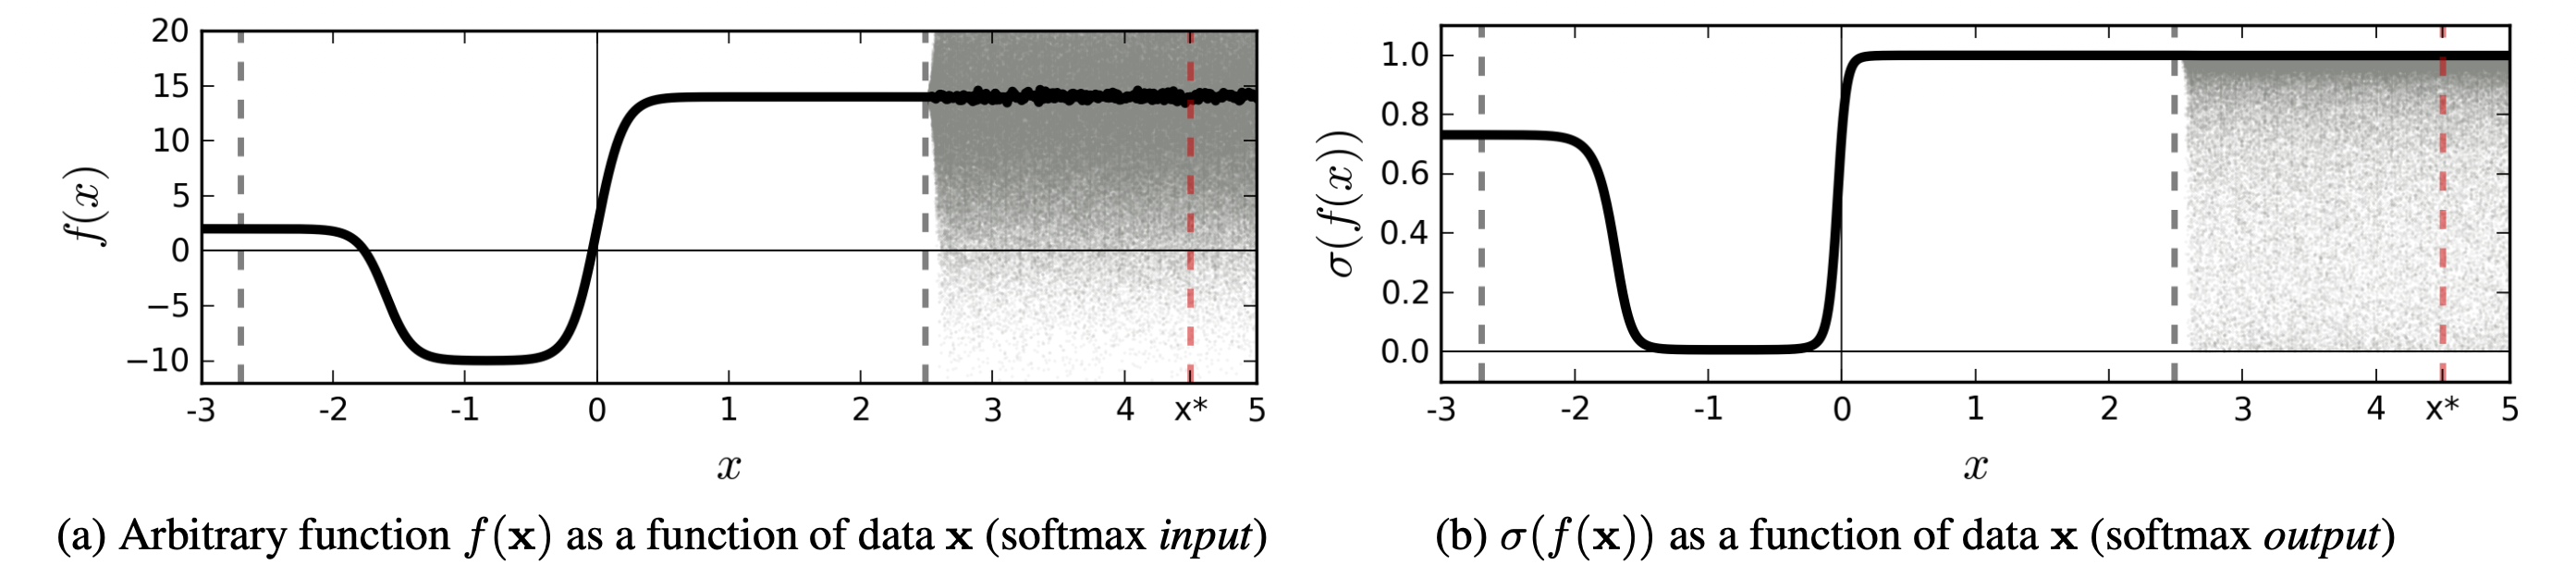
\includegraphics[width=0.75\linewidth]{figure-1.png}
		\caption{A sketch of softmax input and output for an idealised binary classification problem}
	\end{figure}

	\begin{itemize}
		\item Standard deep neural networks produce \alert{point estimates}.
		\item Softmax outputs are often misinterpreted as calibrated confidence.
		\item Far from training data: predictions remain \alert{highly confident}.
		\item Missing: \textbf{epistemic uncertainty} (model uncertainty).
	\end{itemize}
\end{frame}

%------------------------------------------------

\subsection{Classical Dropout vs Bayesian Neural Networks}

\begin{frame}
	\frametitle{Classical Dropout vs Bayesian Neural Networks}

	\begin{columns}[t]
		\begin{column}{0.48\textwidth}
			\textbf{Bayesian Neural Networks}
			\begin{itemize}
				\item Prior over weights: $p(\omega)$
				\item Posterior:
				\[
				p(\omega|X,Y)
				\]
				\item Intractable for deep NNs
				\item MCMC (Gibbs, HMC) expensive
				\item This motivates \alert{approximate inference}
			\end{itemize}
		\end{column}

		\begin{column}{0.48\textwidth}
			\textbf{Classical Dropout}
			\begin{itemize}
				\item Randomly zero activations
				\item Prevents co-adaptation
				\item Interpreted as heuristic regularizer
				\item No explicit probabilistic view
				\item Can we view \alert{dropout} as approximate \alert{Bayesian} inference?
			\end{itemize}
		\end{column}
	\end{columns}
\end{frame}

\subsection{Dropout as Model Averaging}

\begin{frame}
	\frametitle{Dropout as Approximate Model Averaging}

	\begin{itemize}
		\item Each dropout mask defines a \alert{sub-network}.
		\item With $K$ units per layer $\Rightarrow 2^K$ possible subnetworks.
		\item Training with dropout implicitly trains an ensemble of networks
		with shared weights.
	\end{itemize}

	\bigskip
	
	\textbf{Bayesian Perspective:}
	
	True predictive distribution:
	\[
	p(y^*|x^*,X,Y)
	=
	\int p(y^*|x^*,\omega)p(\omega|X,Y)d\omega
	\]

	\bigskip
	
	Dropout approximation:
	\[
	p(y^*|x^*) \approx
	\frac{1}{T}\sum_{t=1}^T
	p(y^*|x^*,\omega_t)
	\]

\end{frame}

%----------------------------------------------------------------------------------------
%	SECTION 2
%----------------------------------------------------------------------------------------

\section{Dropout as Variational Inference}

%------------------------------------------------
\subsection{Core Insight}

\begin{frame}
	\frametitle{Dropout = Variational Inference}

	\textbf{Variational Objective:}
	\[
	\mathcal{L}_{VI}
	=
	-\int q(\omega)\log p(Y|X,\omega)d\omega
	+
	\text{KL}(q(\omega)||p(\omega))
	\]

	\bigskip

	\begin{itemize}
		\item Dropout training $\equiv$ approximate VI in a deep Gaussian Process.
		\item Approximate posterior:
		\[
		q(\omega)
		\]
		\item Bernoulli variational family:
		\[
		W_i = M_i \cdot \text{diag}(z_{i,j})
		\]
		\[
		z_{i,j} \sim \text{Bernoulli}(p_i)
		\]
	\end{itemize}

\end{frame}

%------------------------------------------------

\subsection{ELBO Perspective}

\begin{frame}
	\frametitle{Optimizing the ELBO}

	\textbf{Standard Dropout Objective:}
	\[
	\mathcal{L}_{dropout}
	=
	\frac{1}{N}\sum_{i=1}^N E(y_i,\hat{y}_i)
	+
	\lambda \sum_{i=1}^L (||W_i||_2^2 + ||b_i||_2^2)
	\]

	\bigskip

	\textbf{Dropout as Variational Approximation:}
		\[
		\mathcal{L}_{GP-MC} 
		\propto 
		\frac{1}{N} \sum_{n=1}^{N} 
		\frac{- \log p(y_n \mid x_n, \hat{\omega_n})}{\tau} +
		\sum_{i=1}^{L}\Big( \frac{p_il^2}{2\tau N}||M_i||_2^2 + \frac{l^2}{2\tau N}||m_i||^2_2\Big)
		\]

	\bigskip


	\begin{itemize}
		\item $L_2$ regularization $\leftrightarrow$ Gaussian prior
		\item Training minimizes KL divergence to posterior
		\item Equivalent to maximizing the ELBO
		\item \alert{Standard dropout loss} is equivalent to the \alert{negative ELBO}
	\end{itemize}

\end{frame}

\begin{frame}
	\frametitle{Connection to Deep Gaussian Processes}

	\begin{itemize}
		\item Single-layer NN with infinite width $\Rightarrow$ Gaussian Process.
		\item Dropout introduces multiplicative Bernoulli noise.
		\item This induces a variational approximation to a Deep GP posterior.
	\end{itemize}

	\bigskip
	
	\[
	f^{(l)}(x)
	=
	W^{(l)} \sigma(f^{(l-1)}(x))
	\]

	Under dropout:
	\[
	W^{(l)} = M^{(l)} \cdot \text{diag}(z)
	\]

	\begin{itemize}
		\item Random masks approximate integrating over function space.
	\end{itemize}

\end{frame}

%----------------------------------------------------------------------------------------
%	SECTION 3
%----------------------------------------------------------------------------------------

\section{Monte Carlo Dropout}

%------------------------------------------------
\subsection{MC Approximation}

\begin{frame}
	\frametitle{Monte Carlo Dropout}

	\begin{itemize}
		\item Keep dropout \alert{active} at test time.
		\item Perform $T$ stochastic forward passes and average them.
		\item Approximate intractable posterior predictive distribution.
	\end{itemize}

	\bigskip

	\textbf{Predictive Mean:}
	\[
	\mathbb{E}[y^*]
	\approx
	\frac{1}{T}\sum_{t=1}^{T}\hat{y}^{*t}
	\]

	\textbf{Predictive Variance:}
	\[
	\text{Var}(y^*)
	\approx
	\tau^{-1}I
	+
	\frac{1}{T}\sum_{t=1}^{T}
	\hat{y}^{*t}\hat{y}^{*tT}
	-
	\mathbb{E}[y^*]\mathbb{E}[y^*]^T
	\]

	\begin{itemize}
	\item Variance term captures \alert{epistemic uncertainty}.
	\item $\tau^{-1} I$ captures model precision (linked to prior).
	\item Uncertainty increases far from training data.
\end{itemize}
\end{frame}

%----------------------------------------------------------------------------------------
%	SECTION 4
%----------------------------------------------------------------------------------------

\section{Empirical Results and Insights}

\subsection{Quantitative Evaluation}

\begin{frame}
\frametitle{Predictive Log-Likelihood and RMSE Comparison}

\begin{figure}
    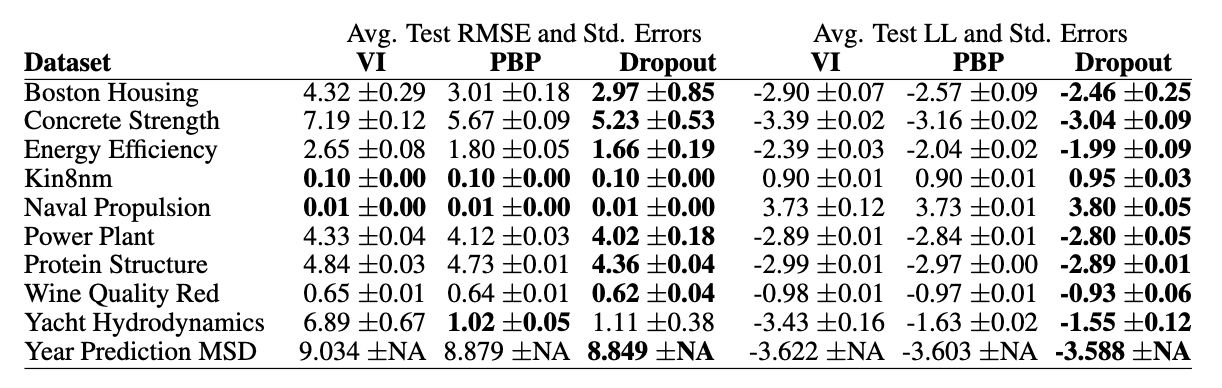
\includegraphics[width=0.75\linewidth]{table-1.png}
    \caption{Predictive performance (RMSE and Log-Likelihood) across VI, PBP, and MC Dropout. MC Dropout achieves competitive RMSE and higher log-likelihood, showing better uncertainty estimation.}
\end{figure}

\begin{itemize}
    \item Demonstrates principled Bayesian behavior.
    \item RMSE shows accuracy, Log-Likelihood shows calibrated uncertainty.
    \item BO (Bayesian Optimization) further improves performance.
\end{itemize}

\end{frame}

%------------------------------------------------
\subsection{Task-Level Demonstration}

	\begin{frame}
		\frametitle{MC Dropout in Action}

		\begin{columns}[t]


		% Regression
		\begin{column}{0.48\textwidth}
		\begin{figure}
				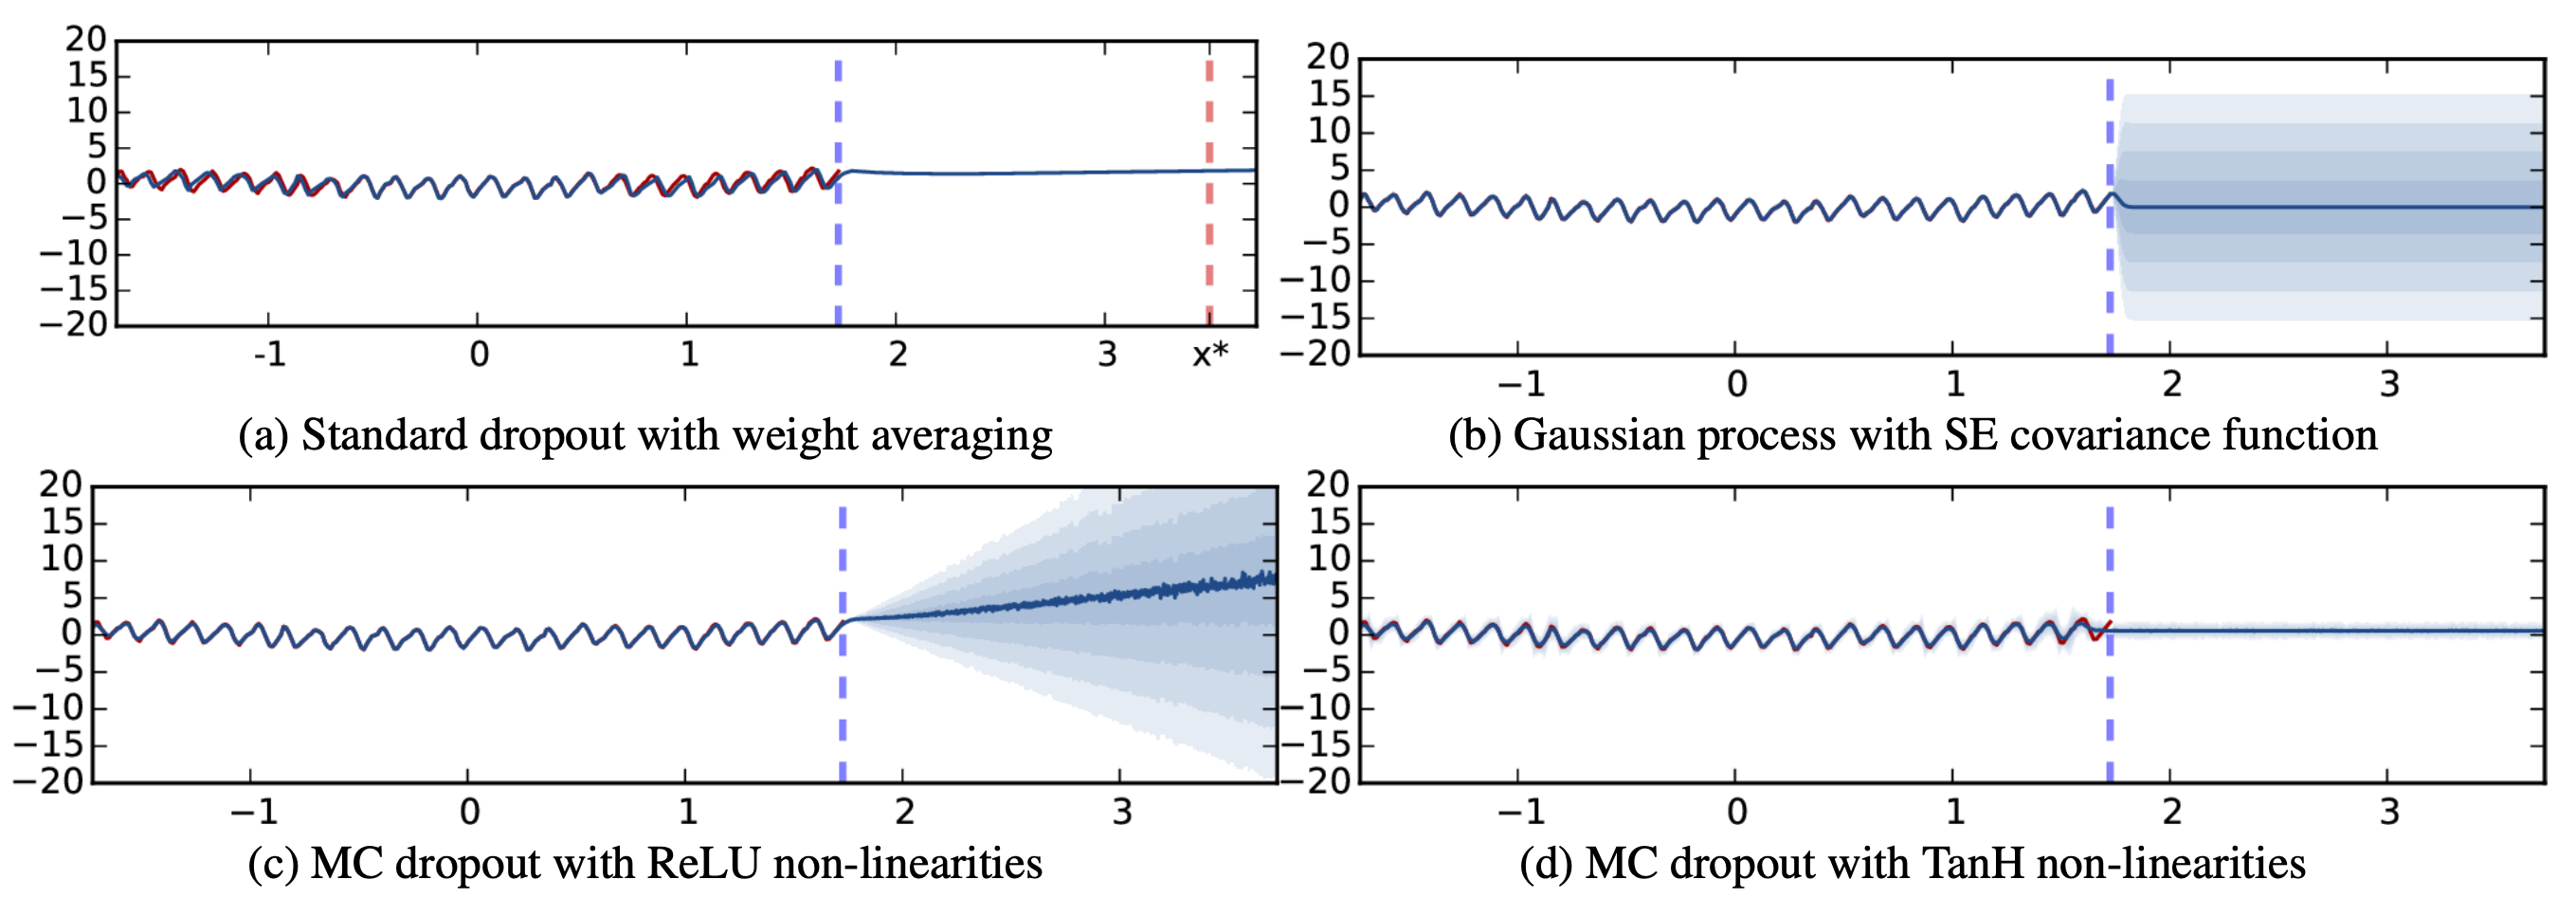
\includegraphics[width=\linewidth,height=0.2\textheight,keepaspectratio]{figure-2.png}
				\caption{Regression: predictive mean $\pm$ uncertainty.}
		\end{figure}
		\end{column}

		% Classification
		\begin{column}{0.48\textwidth}
		\begin{figure}
				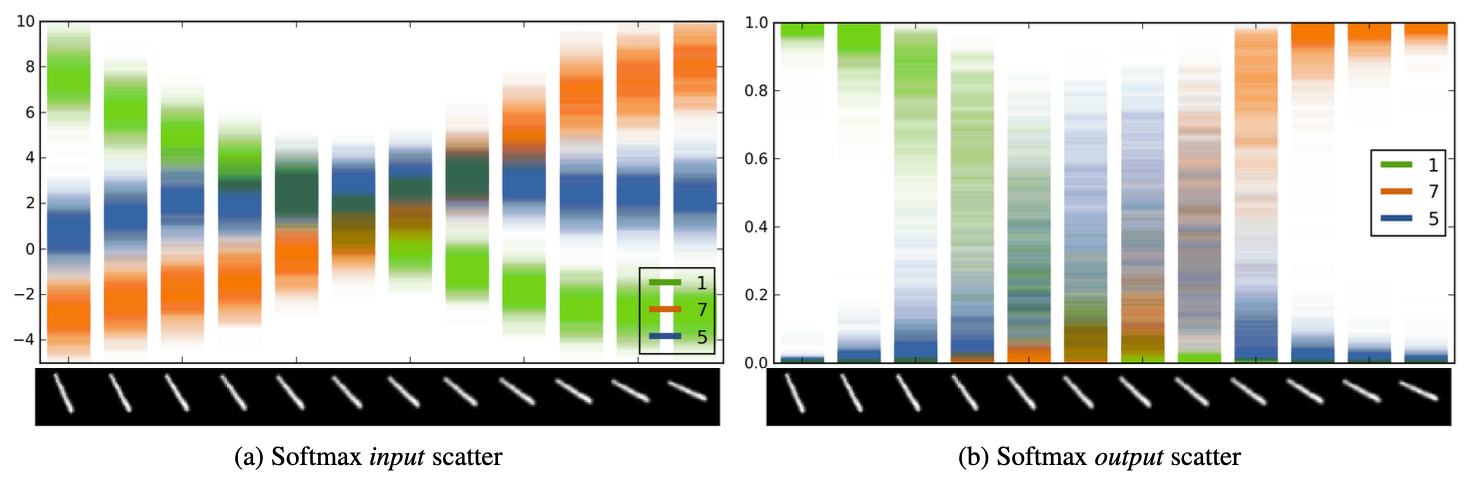
\includegraphics[width=\linewidth,height=0.2\textheight,keepaspectratio]{figure-4.png}
				\caption{Classification: softmax uncertainty on rotated digits.}
		\end{figure}
		\end{column}

		\end{columns}

		\begin{center}
		\begin{figure}
		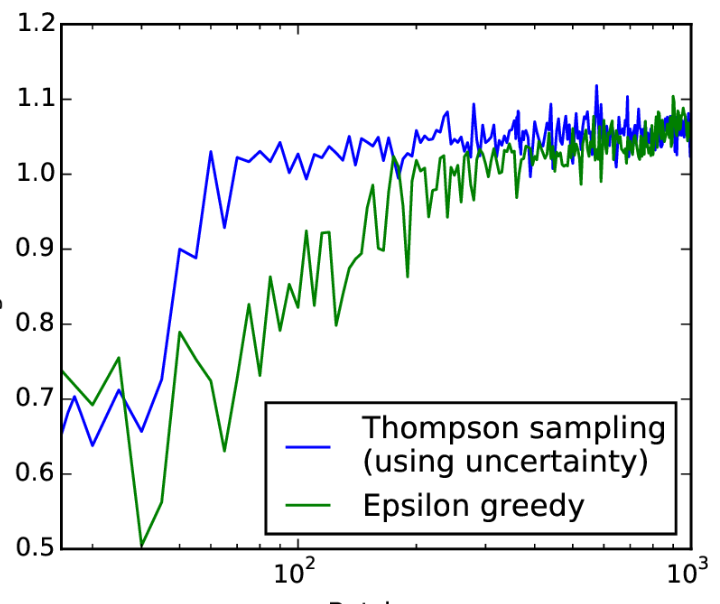
\includegraphics[width=0.6\linewidth,height=0.3\textheight,keepaspectratio]{figure-6.png}
		\caption{RL: MC Dropout (Thompson sampling) vs $\epsilon$-greedy average reward.}
		\end{figure}
		\end{center}



	\end{frame}

%------------------------------------------------
\subsection{Why This is Powerful}

\begin{frame}
	\frametitle{Why MC Dropout is Powerful}
	Dropout casts Bayesian inference as a fast optimization problem rather than a sampling problem.
	\begin{itemize}
		\item Uncertainty estimates using existing models.
		\item No doubled parameterization.
		\item No burn-in.
		\item Scales to modern deep architectures.
	\end{itemize}

	\bigskip
	\textbf{Trade-off:}
	\begin{itemize}
		\item VI: fast, biased (mode-seeking).
		\item MCMC: accurate, computationally heavy.
	\end{itemize}

\end{frame}

%------------------------------------------------
\subsection{Conclusion and Limitations}

\begin{frame}
	\frametitle{Conclusion and Limitations}

	\begin{block}{Conclusion}
		\begin{itemize}
			\item Dropout reinterpreted as approximate Bayesian inference.
			\item Provides fast, scalable uncertainty estimation.
		\end{itemize}
	\end{block}

	\begin{alertblock}{Limitations}

	\begin{itemize}
		\item Variational family is mean-field Bernoulli: cannot represent multimodal posteriors.
		\item KL$(q||p)$ is mode-seeking: underestimates posterior variance.
		\item Prior is implicitly tied to weight decay coefficient.
		\item Approximation quality depends on dropout rate choice.
	\end{itemize}

	\end{alertblock}

\end{frame}

%----------------------------------------------------------------------------------------
%	REFERENCES
%----------------------------------------------------------------------------------------

\section{References}

\begin{frame}
	\frametitle{References}
	
	\footnotesize
	
	Yarin Gal and Zoubin Ghahramani (2016) \\
	\textit{Dropout as a Bayesian Approximation: Representing Model Uncertainty in Deep Learning} \\
	
\end{frame}

%----------------------------------------------------------------------------------------

\end{document} 